% =====================================================================
%  Informe · Módulo "Valoraciones y reseñas de escenarios" · PDF 7
%  Examen Práctico Integrador · Desarrollo de Aplicaciones Móviles
%  Compilar: latexmk -pdf informe-valoraciones.tex
% =====================================================================
\documentclass[11pt,a4paper]{article}

\usepackage[utf8]{inputenc}
\usepackage[T1]{fontenc}
\usepackage[spanish]{babel}
\usepackage{lmodern}
\usepackage[margin=2.4cm]{geometry}
\usepackage{graphicx}
\usepackage{booktabs}
\usepackage{longtable}
\usepackage{array}
\usepackage[table,xcdraw]{xcolor}
\usepackage{tcolorbox}
\usepackage{amssymb}
\usepackage{caption}
\usepackage{verbatim}
\usepackage[colorlinks=true,linkcolor=blue!55!black,urlcolor=blue!55!black,citecolor=blue!55!black]{hyperref}

\graphicspath{{../GUia-Examen/evidencias/}}
\newcommand{\ok}{\textcolor{green!50!black}{\checkmark}}

\begin{document}

\begin{center}
{\LARGE\bfseries Módulo ``Valoraciones y reseñas de escenarios''}\\[0.6em]
{\large Examen Práctico Integrador --- PDF 7: Nuevo módulo / funcionalidad}\\[0.4em]
\textbf{Proyecto:} Lugares Interactivos --- Visualización interactiva de escenarios deportivos a nivel nacional\\[0.3em]
\textbf{App:} Expo / React Native (expo-router, Supabase, react-query, react-hook-form + Zod)\\
\textbf{Rama:} Examen-NicolasReguerin \\[0.5em]
\today
\end{center}

\vspace{0.6em}
\begin{tcolorbox}[colback=blue!8!white,colframe=blue!70!black,arc=2mm,boxrule=1pt]
\centering
\large\bfseries Código fuente disponible en GitHub\\[0.4em]
\normalsize
\href{https://github.com/Joaquinfr87/proyecto-movil/tree/ExamenFinalNicolasReguerin}
      {github.com/Joaquinfr87/proyecto-movil }\\
\emph{Rama:} \texttt{ExamenFinalNicolasReguerin}
\end{tcolorbox}

\section{Funcionalidad implementada}
\label{sec:funcionalidad}

Los usuarios autenticados pueden calificar cada escenario deportivo con \textbf{1 a 5 estrellas}
y dejar un comentario opcional. La aplicación permite:

\begin{itemize}
  \item Ver el \textbf{promedio} y la \textbf{cantidad} de valoraciones de cada escenario
        (en el detalle y en las tarjetas del catálogo).
  \item Ver la \textbf{lista de reseñas} con el autor y su comentario.
  \item Gestionar desde la pestaña \emph{Valoraciones} las \textbf{mis valoraciones}
        (consultar, editar o eliminar).
\end{itemize}

\section{Problema o necesidad que resuelve}
\label{sec:problema}

La app ofrece información oficial de infraestructura deportiva (capacidad, horario, fotos,
eventos), pero el usuario no disponía de información sobre la \textbf{experiencia y el estado
percibido} de cada escenario. Las valoraciones agregan información comunitaria que ayuda a otros
ciudadanos a decidir y proporciona retroalimentación al personal de gestión.

\section{Usuarios involucrados}
\label{sec:usuarios}

\begin{itemize}
  \item \textbf{Ciudadanía} (rol \texttt{asistente} / cualquier usuario autenticado): valora,
        consulta y gestiona sus propias reseñas.
  \item \textbf{Gestores y administradores}: consultan las valoraciones de los escenarios que
        administran. El \texttt{admin} puede eliminar cualquier valoración (moderación).
\end{itemize}

\section{Objetivo}
\label{sec:objetivo}

Permitir que la comunidad califique los escenarios y consultar el promedio de forma centralizada,
integrada a la navegación existente, sin duplicar datos ni romper la lógica actual.

\section{Flujo de funcionamiento}
\label{sec:flujo}

\begin{verbatim}
  Usuario
    1. Abre el detalle de un escenario (o la pestaña Valoraciones)
    2. Toca "Valorar" / "Editar mi valoración"
    3. Selecciona estrellas (1-5) y escribe un comentario opcional
    4. Se validan los datos (react-hook-form + Zod)
    5. Se guarda en Supabase (upsert por usuario + escenario)
    6. Se recalculan promedio y lista (react-query)
    7. Consulta / edita / elimina desde "Mis Valoraciones" o el detalle
\end{verbatim}

\section{Pantallas creadas y modificadas}
\label{sec:pantallas}

\begin{longtable}{@{}p{6.2cm}p{1.5cm}p{6.5cm}@{}}
\toprule
\textbf{Pantalla / componente} & \textbf{Tipo} & \textbf{Descripción}\\
\midrule
\endhead
\texttt{src/app/(tabs)/ratings.tsx} & Nueva & \emph{Mis Valoraciones}: lista con crear/editar/eliminar\\
\texttt{src/app/(tabs)/\_layout.tsx} & Modificada & Pestaña \emph{Valoraciones} (icono star-half)\\
\texttt{src/app/scenario/[id].tsx} & Modificada & Sección Valoraciones: promedio, botón Valora, reseñas\\
\texttt{components/rating/RatingStars.tsx} & Nueva & Selector / visualización de estrellas\\
\texttt{components/rating/RatingFormModal.tsx} & Nueva & Modal crear/editar valoración (RHF + Zod)\\
\texttt{components/rating/RatingList.tsx} & Nueva & Lista de reseñas con acciones propias\\
\texttt{components/common/ScenarioCard.tsx} & Modificada & Badge de promedio y cantidad\\
\texttt{hooks/useScenarioRatings.ts} & Nueva & CRUD + estadísticas + caché offline\\
\texttt{utils/ratingDraft.ts} & Nueva & Persistencia local (borrador + caché)\\
\bottomrule
\end{longtable}

\section{Base de datos: Supabase / PostgreSQL}
\label{sec:bd}

\subsection{Tabla nueva: \texttt{public.scenario\_ratings}}
Migración \texttt{011\_create\_scenario\_ratings.sql}.

\begin{center}
\begin{tabular}{@{}lll@{}}
\toprule
\textbf{Campo} & \textbf{Tipo} & \textbf{Notas}\\
\midrule
\texttt{id} & UUID PK & \texttt{gen\_random\_uuid()}\\
\texttt{scenario\_id} & UUID FK $\rightarrow$ \texttt{scenarios.id} & \texttt{ON DELETE CASCADE}\\
\texttt{user\_id} & UUID FK $\rightarrow$ \texttt{profiles.id} & \texttt{ON DELETE CASCADE}\\
\texttt{rating} & SMALLINT & \texttt{CHECK (rating BETWEEN 1 AND 5)}\\
\texttt{comment} & TEXT & default \texttt{''}, máx. 500 (validación en app)\\
\texttt{created\_at} / \texttt{updated\_at} & TIMESTAMPTZ & trigger automático\\
\bottomrule
\end{tabular}
\end{center}

\textbf{Restricción única:} \texttt{UNIQUE (user\_id, scenario\_id)} -- una valoración por usuario
y escenario. \textbf{Índices:} por \texttt{scenario\_id} y por \texttt{user\_id}.

\subsection{RLS (Row Level Security)}
\begin{center}
\begin{tabular}{@{}ll@{}}
\toprule
\textbf{Operación} & \textbf{Política}\\
\midrule
SELECT & autenticados y anónimos (el público puede ver reseñas)\\
INSERT & \texttt{user\_id = auth.uid()}\\
UPDATE & \texttt{user\_id = auth.uid()}\\
DELETE & \texttt{user\_id = auth.uid()} o rol \texttt{admin}\\
\bottomrule
\end{tabular}
\end{center}

\subsection{Función: \texttt{public.scenario\_rating\_stats()}}
Devuelve \texttt{(scenario\_id, average, count)} agrupado, usada para el promedio en las tarjetas
del catálogo (\texttt{SECURITY DEFINER}, solo expone agregados).

\section{Operaciones CRUD}
\label{sec:crud}

\begin{center}
\begin{tabular}{@{}lp{4.6cm}p{6.8cm}@{}}
\toprule
\textbf{Operación} & \textbf{Dónde} & \textbf{Cómo}\\
\midrule
Create & detalle / modal & \texttt{upsert} con \texttt{onConflict: user\_id,scenario\_id}\\
Read & detalle y pestaña & \texttt{SELECT} con join a \texttt{profiles} y \texttt{scenarios}\\
Update & modal de edición & \texttt{upsert} (misma clave)\\
Delete & detalle y pestaña & \texttt{DELETE} por id (propia; admin: cualquiera)\\
Aggregate & tarjetas del catálogo & \texttt{rpc('scenario\_rating\_stats')}\\
\bottomrule
\end{tabular}
\end{center}

La UI refleja los cambios al instante invalidando queries de react-query
(\texttt{['scenario-ratings', id]}, \texttt{['my-ratings', userId]}, \texttt{['rating-stats']}).

\section{Persistencia utilizada}
\label{sec:persistencia}

\subsection{Supabase (centralizada)}
Promedios, reseñas y quién las emitió deben ser consultables por todos los usuarios desde
cualquier dispositivo y moderables por \texttt{admin} $\rightarrow$ se almacenan en PostgreSQL
vía Supabase.

\subsection{AsyncStorage (local) -- \texttt{utils/ratingDraft.ts}}
\begin{itemize}
  \item \textbf{Borrador de la valoración} (\texttt{rating\_draft:v1:\{userId\}}): si el usuario
        escribe estrellas / comentario y cierra el modal sin guardar, el borrador se restaura la
        próxima vez.
  \item \textbf{Caché offline de ``Mis Valoraciones''} (\texttt{my\_ratings\_cache:v1:\{userId\}}):
        la pestaña muestra los datos guardados del dispositivo antes de la respuesta del servidor.
\end{itemize}
Justificación: información privada por dispositivo y temporales de edición. El proyecto ya tenía
\texttt{AsyncStorage} instalado pero sin uso; es la primera funcionalidad que lo aprovecha.

\section{Validaciones y manejo de errores}
\label{sec:validaciones}

\begin{itemize}
  \item \textbf{Validación de campos:} Zod en el formulario -- calificación requerida entre 1 y 5;
        comentario opcional con máximo 500 caracteres.
  \item \textbf{Datos inválidos:} el \texttt{CHECK (rating BETWEEN 1 AND 5)} y el
        \texttt{UNIQUE} refuerzan a nivel de base de datos.
  \item \textbf{Información inexistente:} \texttt{EmptyState} (``Sin valoraciones aún'') y estado
        de error con reintento.
  \item \textbf{Error al guardar:} mensaje en el modal sin cerrar el formulario.
  \item \textbf{Error de consulta:} \texttt{ErrorState} con botón ``Reintentar'' en la pestaña.
  \item \textbf{Doble envío:} botón deshabilitado con \emph{spinner} mientras guarda.
\end{itemize}

\section{Pruebas realizadas}
\label{sec:pruebas}

\begin{longtable}{@{}rlp{8.5cm}@{}}
\toprule
\textbf{\#} & \textbf{Prueba} & \textbf{Resultado}\\
\midrule
\endhead
1 & Acceso al módulo (pestaña Valoraciones + botón en detalle) & \ok\\
2 & Ingreso de datos válidos (5 estrellas + comentario) & \ok inserción correcta\\
3 & Ingreso de datos inválidos (\texttt{rating = 6}) & \ok rechazado por CHECK\\
4 & Validación de campos (0 estrellas al publicar) & \ok error en UI\\
5 & Guardado de información (CREATE vía \texttt{upsert}) & \ok\\
6 & Consulta (lista con \texttt{profiles} + promedio por RPC) & \ok\\
7 & Modificación (UPDATE del propio rating / comentario) & \ok\\
8 & Eliminación (DELETE propia) & \ok\\
9 & Persistencia (caché AsyncStorage + borrador) & \ok implementada\\
10 & Manejo de errores (RLS ajeno bloqueado: INSERT/UPDATE/DELETE) & \ok\\
11 & RLS: \texttt{admin} puede eliminar valoración ajena & \ok\\
12 & Estadísticas agregadas (\texttt{scenario\_rating\_stats}) & \ok\\
\bottomrule
\end{longtable}

Las pruebas 1--12 se ejecutaron contra \textbf{Supabase local} (script de \emph{smoke test} con
\texttt{@supabase/supabase-js}): autenticación con usuarios \emph{seed}, CRUD completo,
\emph{constraints} y control de RLS.

\section{Desafío adicional}
\label{sec:desafio}
\begin{itemize}
  \item Ordenamiento de reseñas por más recientes (\texttt{created\_at desc}).
  \item Edición \emph{inline} vía el mismo modal reutilizado (crear/editar/eliminar desde detalle
        y desde la pestaña).
  \item Promedio agregado en tarjetas del catálogo sin duplicar consultas.
  \item Caché offline de ``Mis Valoraciones'' y borrador en AsyncStorage.
\end{itemize}

\section{Dificultades encontradas}
\label{sec:dificultades}
\begin{enumerate}
  \item \textbf{Privilegios de tabla en Supabase local:} las tablas nuevas no recibían los grants
        automáticos (\texttt{authenticated} sin INSERT/SELECT); se agregaron \texttt{GRANT}
        explícitos en la migración.
  \item \textbf{Caché de esquema de PostgREST:} tras aplicar la migración la API devolvía 404
        hasta recargar el esquema (resuelto con \texttt{db reset} y reinicio del contenedor
        \texttt{rest}).
  \item \textbf{Ambigüedad en el listado de migraciones local} que sugería que \texttt{011} estaba
        aplicada cuando no lo estaba; verificado directamente con \texttt{psql}.
  \item \textbf{Tipos de expo-router desactualizados} (\texttt{.expo/types/router.d.ts}):
        errores de TS preexistentes en \texttt{manage.tsx} que se regeneran con \texttt{expo start}.
  \item \textbf{Lint preexistente roto} en el repo (ESLint v10 requiere \emph{flat config} y el repo
        usa \texttt{.eslintrc.js}); se aplicó Prettier y \texttt{tsc} validado sobre los archivos
        del módulo.
\end{enumerate}

\section{Cómo compilar el APK para Android}
\label{sec:demo}

La aplicación se ejecuta desde el proyecto nativo \texttt{android/} de Expo (SDK 57).
Requisitos: JDK 17 y Android SDK (variables \texttt{ANDROID\_HOME} o \texttt{ANDROID\_SDK\_ROOT}
apuntando al SDK).

\begin{enumerate}
  \item Conectar el celular por USB y habilitar la \emph{depuración por USB}.
  \item Verificar la IP de la base: si se usa \textbf{Supabase local}, apuntar en \texttt{.env} a la
        IP de la máquina en la LAN (p.\ ej. \texttt{http://192.168.x.x:54321}) y la \emph{anon key}
        local. En emulador Android usar \texttt{http://10.0.2.2:54321}.
  \item Compilar el APK en modo \texttt{release} (firmado con la \emph{debug key}, instalable):

\begin{verbatim}
cd android
./gradlew assembleRelease
\end{verbatim}

El APK generado queda en
\texttt{android/app/build/outputs/apk/release/app-release.apk} y se instala con:

\begin{verbatim}
adb install app-release.apk
\end{verbatim}

  \item Alternativa con Expo: \texttt{npx expo run:android} compila e instala directamente en el
        dispositivo conectado.
\end{enumerate}

Al acceder por primera vez iniciar sesión con el usuario \emph{seed}:
\texttt{asistente@test.com} / \texttt{password123}.

\section{Evidencias (capturas)}
\label{sec:evidencias}

\begin{figure}[htbp]
\centering
\begin{minipage}[t]{0.45\linewidth}
\centering

\includegraphics[width=\linewidth]{01-tab-valoraciones.png}
\captionof{figure}{Pestaña \emph{Valoraciones} (pantalla principal del módulo).}
\label{fig:tab}
\end{minipage}\hfill
\begin{minipage}[t]{0.45\linewidth}
\centering
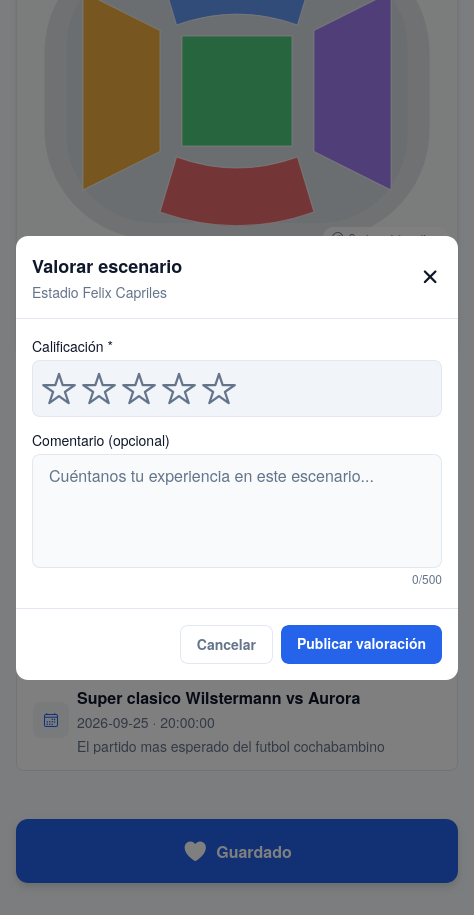
\includegraphics[width=\linewidth]{02-modal-valorar.png}
\captionof{figure}{Modal \emph{Valorar escenario}: estrellas 1--5 + comentario.}
\label{fig:modal}
\end{minipage}
\end{figure}

\begin{figure}[htbp]
\centering
\begin{minipage}[t]{0.45\linewidth}
\centering

\includegraphics[width=\linewidth]{03-detalle-promedio.png}
\captionof{figure}{Sección Valoraciones en el detalle: promedio y reseñas con autor.}
\label{fig:promedio}
\end{minipage}\hfill
\begin{minipage}[t]{0.45\linewidth}
\centering

\includegraphics[width=\linewidth]{04-tarjeta-promedio.png}
\captionof{figure}{Tarjeta del catálogo con badge de promedio y cantidad.}
\label{fig:tarjeta}
\end{minipage}
\end{figure}

\begin{figure}[htbp]
\centering
\begin{minipage}[t]{0.45\linewidth}
\centering

\includegraphics[width=\linewidth]{05-validacion-error.png}
\captionof{figure}{Validación de campos (error al publicar sin estrellas).}
\label{fig:validacion}
\end{minipage}\hfill
\begin{minipage}[t]{0.45\linewidth}
\centering
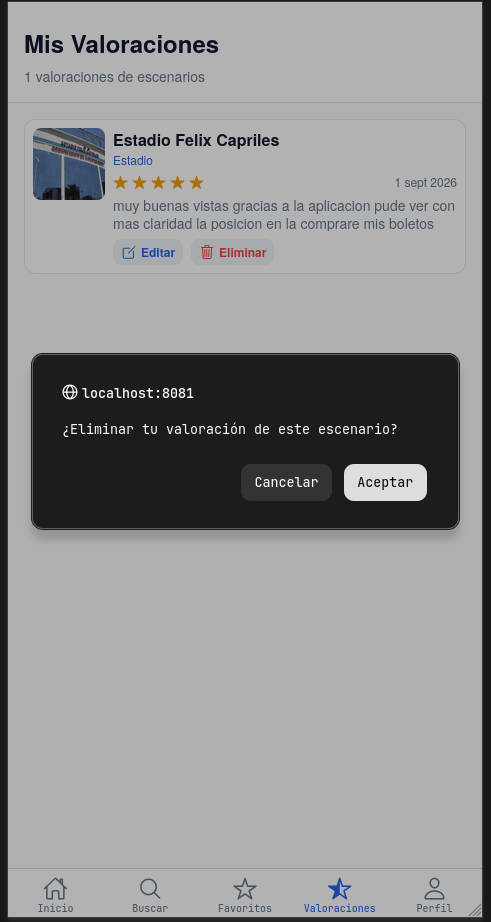
\includegraphics[width=\linewidth]{06-eliminar-valoracion.png}
\captionof{figure}{Confirmación de eliminación de una valoración.}
\label{fig:eliminar}
\end{minipage}
\end{figure}

\begin{figure}[htbp]
\centering

\includegraphics[width=0.55\linewidth]{07-boton-valorar-en-detalle.png}
\captionof{figure}{Acceso al módulo desde el detalle del escenario.}
\label{fig:acceso}
\end{figure}

\end{document}